\section*{Statistical Approaches for Outlier Detection}
Statistical methodologies for anomaly detection operate on a different fundamental logic than the representation learning approaches previously discussed. 
These methods characterize the underlying distribution of the data to estimate population parameters, such as the mean and covariance. 
This allows for statistical inference, wherein the model assigns a probability to each data point, quantifying the likelihood that it constitutes an outlier.


In a multivariate dataset, the covariance matrix is a critical parameter as it defines the geometric shape and orientation of the data within a p-dimensional space. 
Consequently, utilizing the Mahalanobis distance %\refeq:mahalanobis) is highly advantageous, as it incorporates this covariance to measure distances in a scale-invariant manner. \todo{proof}
A naive approach to outlier detection would involve estimating the sample mean and covariance matrix for the entire dataset and labeling the $n$ observations with the largest Mahalanobis distances as outliers.


However, this standard procedure is often compromised by the masking effect. 
Because classical estimators for the mean and covariance are highly sensitive to extreme values, even a single outlier can shift the mean toward itself and artificially inflate the covariance. 
This effectively "masks" the outlier’s presence, leading to false negatives. 
To address this, the Minimum Covariance Determinant (MCD) was proposed by \citet{rousseeuw1984least} and theoretically formalized in \citet{rousseeuw1985multivariate} to provide robust estimators that remain unaffected by data contamination.

\begin{figure}[h] 
    \centering
    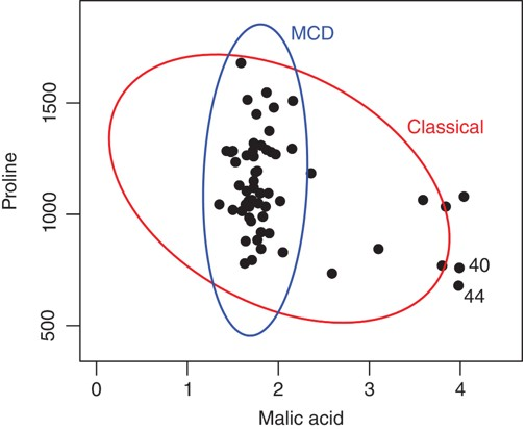
\includegraphics[width=0.6\linewidth]{Images/MCD.pdf}
    \caption{grapfical depiction of the Minimum Covariance Determinant}
    \label{fig:mcd}
\end{figure}

\subsection*{Minimum Covariance Determinant (MCD)}
The objective of the MCD is to identify a subset $H$ containing $h$ observations that yields the minimum possible covariance matrix determinant.
Geometrically, the MCD seeks the smallest possible ellipsoid that encapsulates a specific fraction of the data. \todo{which one is right?}  
By drawing this ellipsoid around the region of highest local density rather than the entire dataset, the MCD effectively excludes outliers and eliminates the masking effect.


The MCD is characterized by a high breakdown point, which is the maximum proportion of arbitrarily large outliers a dataset can contain before the estimator produces unreliable results. 
Under the so called majority rule, the MCD remains consistent even if up to 50\% of the data points are outliers, provided the algorithm identifies the correct h-subset. 
If the outlier ratio exceeds 50\%, these points can no longer be statistically defined as outliers, as they constitute the majority class.
Furthermore, the MCD is affine equivariant, meaning the estimators remain consistent under affine transformation changes such as scaling, rotation, or translation that preserve the data's structural integrity \citet{hubert2018minimum}. 
Unlike k-NN or deep learning models, which require careful normalization, MCD estimators are naturally robust to these kinds of transformations.


\section*{FAST-MCD}
A significant limitation of the original MCD algorithm is its computational complexity. 
Finding the optimal subset requires evaluating $\binom{n}{h}$ combinations, which is infeasible for large datasets. 
To resolve this, \citet{rousseeuw1999fast} introduced the FAST-MCD algorithm, which utilizes concentration steps (C-Steps) to iteratively improve the subset selection:


\begin{enumerate}
\item  Determine the subset size $h$, using the formula $h = \frac{2n + p + 1}{2}$.
\item Perform initial C-Steps on several random subsamples.
\item Select the ten results with the lowest determinants ($det(S)$) and continue C-Steps until convergence.
\item  Report the mean ($\mu^MCD$) and covariance ($\Sigma^MCD$) from the subset with the overall lowest determinant
\end{enumerate}


The C-Step operates by calculating the Mahalanobis distances for all $n$ observations based on a current subset's parameters, then forming a new subset from the $h$ observations with the smallest distances. 
This process is guaranteed to decrease the determinant of the covariance matrix at each iteration until convergence \citep[p.214]{rousseeuw1999fast}.\todo{why does it converge?}


\begin{enumerate}
    \item Initialize by drawing a random number $p+1$ subsamples $J$ and calculate the sample mean and the sample covariance matrix. If the resulting $det(S0)=0$ then add another random observation until $det(S0)>0$.
    \item If $det(S1)=/0$ compute the mahalanobis distances for all $n$
    \item To compute $H2$ sort the distances of (2) from smallest to biggest
    \item Select the $h$ smallest distances and compute the mean and coverance matrix
    \item Repeat until convergence
\end{enumerate}
\citep[p.214]{rousseeuw1999fast}


\subsection*{Implementation}
In this implementation, two concentration steps will be applied to all initial subsets, followed by a full convergence of the ten most promising candidates. 
This selective iteration is efficient because the distinction between robust and non-robust solutions usually manifests within the first few steps. \todo{add:rousseeuw, Driessen (1999)p.216 pp...} 
If the outlier ratio is known to be below 25\%, choosing h=0.75n offers an optimal balance between robustness (breakdown value) and statistical efficiency.


\section*{Hyperparameter Selection}
The primary hyperparameter for MCD is $h$, constrained by the range:

\begin{equation}
\frac{n+p+1}{2} \le h \le n.
\end{equation}

If $h$ is smaller than the number of dimensions $p$, the covariance matrix becomes singular $det(S)=0$, rendering it non-invertible.
To avoid excessive noise, it is recommended to maintain at least five observations per dimension \citep{hubert2018minimum}.
\todo{right place?}

Once the robust estimators $\mu^MCD$ and $\Sigma^MCD$ are calculated, the Robust Mahalanobis Distance (RD) \todo{true?} is computed for each observation:

\begin{equation}
RD_i^2 = (\mathbf{x}_i - \hat{\mu}_{\text{MCD}})^T \hat{\Sigma}_{\text{MCD}}^{-1} (\mathbf{x}_i - \hat{\mu}_{\text{MCD}})
\label{eq:robust_mahalanobis}
\end{equation}


Assuming the clean data follows a multivariate normal distribution, RD2 follows a $\chi^2$ distribution.
This allows for a formal discordancy test: if RD2 exceeds a critical threshold defined by a significance level $\alpha$, the point is flagged as an outlier. 
Increasing $\alpha$ expands the decision ellipsoid, requiring outliers to be further from the center to be detected.

For this thesis, a fixed threshold approach is used to ensure comparability with the other methods. 
The MCD will rank all observations by their robust distance, and the top n% will be classified as outliers based on the known outlier ratio of the experiments.


\section*{Variants and Evaluation}
Recent advancements include Deterministic MCD (DetMCD), which replaces the random initial subsets of FAST-MCD with a deterministic selection process \citep{hubert2012deterministic}. 
DetMCD is permutation-invariant, meaning the results are independent of data order, and it typically offers faster execution and lower sensitivity to contamination.


In summary, the MCD is defined by its high breakdown point and affine equivariance, which ensures reliability without the need for normalization. 
It effectively solves the masking problem and provides transparent, quantifiable results through probability-based scoring. 
However, it remains computationally demanding, assumes a Gaussian distribution, and is susceptible to the Curse of Dimensionality if n is not sufficiently larger than p \citep[p.5]{smiti2020critical}.


MCD serves as a critical benchmark in this study. 
Its statistical nature provides a baseline to determine whether a dataset necessitates complex machine learning models like InterCont, or if traditional robust statistics are sufficient. 
Furthermore, comparing the affine equivariant MCD against non-equivariant methods will yield insights into how InterCont captures the underlying geometry of the data. \todo{achtung mit dieser aussage}